\documentclass[12pt,landscape]{article}
\usepackage{multicol}
\usepackage{calc}
\usepackage{ifthen}
\usepackage[landscape]{geometry}
\usepackage{amsmath,amsthm,amsfonts,amssymb}
\usepackage{color,graphicx,overpic}
\usepackage{hyperref}
\usepackage{enumitem}
\usepackage{upgreek}
\usepackage{physics}
\usepackage{newtxtext,newtxmath}

% This sets page margins to .5 inch if using letter paper, and to 1cm
% if using A4 paper. (This probably isn't strictly necessary.)
% If using another size paper, use default 1cm margins.
\ifthenelse{\lengthtest { \paperwidth = 11in}}
	{ \geometry{top=.5in,left=.5in,right=.5in,bottom=.5in} }
	{\ifthenelse{ \lengthtest{ \paperwidth = 297mm}}
		{\geometry{top=1cm,left=1cm,right=1cm,bottom=1cm} }
		{\geometry{top=1cm,left=1cm,right=1cm,bottom=1cm} }
	}

% Turn off header and footer
\pagestyle{empty}
 

% Redefine section commands to use less space
\makeatletter
\renewcommand{\section}{\@startsection{section}{1}{0mm}%
                                {-1ex plus -.5ex minus -.2ex}%
                                {0.5ex plus .2ex}%x
                                {\normalfont\normalsize\bfseries}}
\renewcommand{\subsection}{\@startsection{subsection}{2}{0mm}%
                                {-1explus -.5ex minus -.2ex}%
                                {0.5ex plus .2ex}%
                                {\normalfont\small\bfseries}}
\renewcommand{\subsubsection}{\@startsection{subsubsection}{3}{0mm}%
                                {-1ex plus -.5ex minus -.2ex}%
                                {1ex plus .2ex}%
                                {\normalfont\footnotessize\bfseries}}
\renewcommand\small{\@setfontsize\small{10}{11}}                           
\makeatother

% Define BibTeX command
\def\BibTeX{{\rm B\kern-.05em{\sc i\kern-.025em b}\kern-.08em
    T\kern-.1667em\lower.7ex\hbox{E}\kern-.125emX}}

% Don't print section numbers
\setcounter{secnumdepth}{0}

\setlength{\parindent}{0pt}
\setlength{\parskip}{1pt plus 0.5ex}

\newcommand{\tab}{\hspace{.02\textwidth}}
\newcommand{\ds}{\displaystyle}

\def\rcurs{{\mbox{$\resizebox{.09in}{.08in}{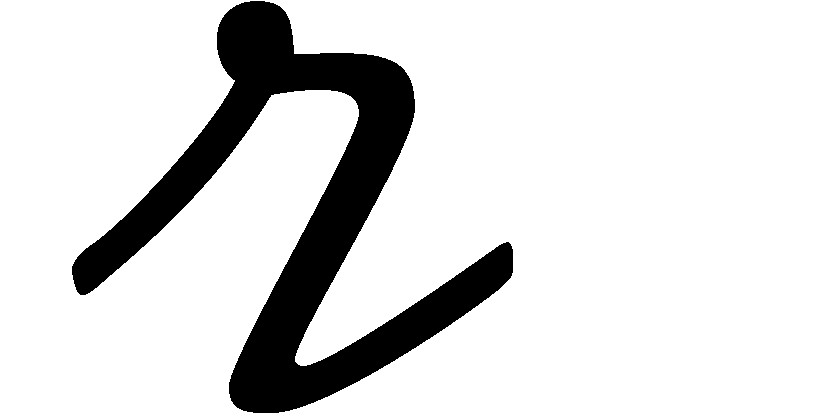
\includegraphics[trim= 1em 0 14em 0,clip]{ScriptR}}$}}}
\def\brcurs{{\mbox{$\resizebox{.09in}{.08in}{
\includegraphics[trim= 1em 0 14em 0,clip]{BoldR}}$}}}

\renewcommand{\dv}[2]{\frac{d#1}{d#2}}

% Redefine some commands for newtxmath boldness
\renewcommand{\grad}{\nabla}
\renewcommand{\curl}[1]{\nabla\times#1}
\renewcommand{\div}[1]{\nabla\cdot#1}
\renewcommand{\cross}{\times}

% -----------------------------------------------------------------------

\begin{document}

\raggedright
\footnotesize
\begin{multicols}{3}


% multicol parameters
% These lengths are set only within the two main columns
%\setlength{\columnseprule}{0.25pt}
\setlength{\premulticols}{1pt}
\setlength{\postmulticols}{1pt}
\setlength{\multicolsep}{1pt}
\setlength{\columnsep}{2pt}

\begin{center}
	\Large{\underline{PHYS 401 Formula Sheet}}
\end{center}

\section{Differential Maxwell's Equations}
\hspace{3mm}\begin{tabular}{p{2cm}p{4cm}}
	$\ds \div{\vb{E}} = \frac{\rho}{\varepsilon_0}$ & $\ds \curl{\vb{E}} = -\pdv{\vb{B}}{t}$\\
	$\ds \div{\vb{B}} = 0$ & $\ds \curl{\vb{B}} = \mu_0\vb{J} + \mu_0\varepsilon_0\pdv{\vb{E}}{t}$
\end{tabular}

\section{Integral Maxwell's Equations}

\begin{tabular}{p{2.75cm}p{5cm}}
	$\ds \oint \vb{E}\cdot d\vb{a} = \frac{Q_\text{enc}}{\varepsilon_0}$ & $\ds \oint \vb{B}\cdot d\vb{a} = 0$\\
	$\ds \oint \vb{E}\cdot d\vb{l} = -\dv{\Phi_B}{t}$ & $\ds \oint \vb{B}\cdot d\vb{l} = \mu_0 I_\text{enc} + \varepsilon_0\mu_0 \dv{\Phi_E}{t}$
\end{tabular}

\section{Electromagnetic Waves}
Wave Speed:\\
\tab $v = \frac{1}{\sqrt{\mu\varepsilon}} = c/n$

Poynting Vector:\\
\tab $\vb{S} = \frac{1}{\mu}\vb{E}\cross\vb{B}$

Momentum Density:\\
\tab $\ds \ds \vb{P} = \frac{1}{c^2}\vb{S}$

Energy per unit volume:\\
\tab $u = \frac{1}{2}\left(\varepsilon\abs{\vb{E}}^2 + \frac{\abs{\vb{B}}^2}{\mu}\right)$

Intensity:\\
\tab $I = \langle \vb{S}\cdot\vu{n}\rangle$

Potentials:\\
\tab $\ds \vb{E} = -\grad{V} - \pdv{\vb{A}}{t} \qquad \vb{B} = \curl{\vb{B}}$

Gauge Transformation:\\
\tab $\ds \vb{A^\prime} = \vb{A} + \grad{\Lambda} \qquad V^\prime = V - \pdv{\Lambda}{t}$

Lorentz Gauge:\\
\tab $\ds \div{\vb{A}} + \mu\varepsilon\pdv{V}{t} = 0$

Lorentz Transformation:\\
\tab $\ds \mu\varepsilon\pdv[2]{\vb{A}}{t} - \laplacian{\vb{A}} = \mu\vb{J}$\\
\tab $\ds \mu\varepsilon\pdv[2]{V}{t} - \laplacian{V} = \frac{\rho}{\varepsilon}$

\section{Plane Waves}
$\vb{E} = \vb{E}_0e^{i(\vu{k}\cdot\vu{r} - \omega t)} \qquad \vb{B} = \vb{B}_0e^{i(\vu{k}\cdot\vu{r} - \omega t)}$

Phase and Group Velocity:\\
\tab $\ds v_p = \frac{\omega}{k} \qquad \ds v_g = \dv{\omega}{k}$

\columnbreak

Magnetic Field from Electric Field:\\
\tab $\ds \vb{B}_0 = \frac{\vb{k}\cross\vb{E}_0}{\omega}$

Intensity:\\
\tab $I = \frac{1}{2}v\varepsilon E_0^2$

Law of Refraction:\\
\tab $\theta_I = \theta_R$

Snell's Law:\\
\tab $n_I \sin\theta_I = n_T\sin\theta_T$

Complex Index of Refraction:\\
\tab $\ds n \approx \sqrt{\varepsilon_r} = n_R + in_I$

Reflection and Transmission Coefficients:\\
\tab $\ds R = \frac{I_R}{I_I} = \frac{I^\text{beam}_R\cos\theta_R}{I^\text{beam}_I\cos\theta_I} =\frac{I^\text{beam}_R}{I^\text{beam}_I}$\\
\tab $\ds T = \frac{I_T}{I_I} = \frac{I^\text{beam}_T\cos\theta_T}{I^\text{beam}_I\cos\theta_I}$

Misc. Constants:\\
\tab $\ds \alpha = \frac{\cos\theta_T}{\cos\theta_I} \qquad \beta = \frac{\mu_1 v_1}{\mu_2 v_2}$


\subsection{Boundary Conditions}
\hspace{3mm}\begin{tabular}{p{3cm}p{4cm}}
	$\bullet \; \varepsilon_1\vb{E}_1^\perp = \varepsilon_2\vb{E}_2^\perp$ & $\bullet \;\vb{E}_1^\parallel = \vb{E}_2^\parallel$\\
	$\bullet \;\vb{B}_1^\perp = \vb{B}_2^\perp$ & $\bullet \;\ds \frac{\vb{B}_1^\parallel}{\mu_1} = \frac{\vb{B}_2^\parallel}{\mu_2}$
\end{tabular}

\subsection{$\vb{E}$ Parallel to Plane of Incidence}
\tab $\vb{k}_I = k_I(\cos\theta_I\vu{z} + \sin\theta_I\vu{x})$\\
\tab $\vb{E}_I = E_Ie^{i[k_I(\cos\theta_I z + \sin\theta_I x) - \omega t]}(\cos\theta_I\vu{x}-\sin\theta_I\vu{z})$\\
\tab $\vb{k}_R = k_I(-\cos\theta_R\vu{z} + \sin\theta_R\vu{x})$\\
\tab $\vb{E}_R = E_Re^{i[k_R(-\cos\theta_R z + \sin\theta_R x) - \omega t]}(\cos\theta_R\vu{x} + \sin\theta_R\vu{z})$\\
\tab $\vb{k}_T = k_T(\cos\theta_T\vu{z} + \sin\theta_T\vu{x})$\\
\tab $\vb{E}_T = E_Te^{i[k_T(\cos\theta_T z + \sin\theta_T x) - \omega t]}(\cos\theta_T\vu{x} - \sin\theta_T\vu{z})$

Field Magnitudes (Fresnel Equations):\\
\tab $\ds \frac{E_R}{E_I} = \left(\frac{\alpha-\beta}{\alpha + \beta}\right) \qquad \frac{E_T}{E_I} = \left(\frac{2}{\alpha + \beta}\right)$

Reflection and Transmission Coefficients:\\
\tab $\ds R = \left(\frac{\alpha-\beta}{\alpha+\beta}\right)^2 \qquad T = \alpha\beta\left(\frac{2}{\alpha + \beta}\right)^2$

Brewster's Angle (no reflected wave, $\alpha = \beta$):\\
\tab $\tan\theta_B = n_2/n_1$

\subsection{$\vb{E}$ Perpendicular to Plane of Incidence}
\tab $\vb{k}_I = k_I(\cos\theta_I\vu{z} + \sin\theta_I\vu{x})$\\
\tab $\vb{B}_I = B_Ie^{i[k_I(\cos\theta_I z + \sin\theta_I x) - \omega t]}(-\cos\theta_I\vu{x}+\sin\theta_I\vu{z})$\\
\tab $\vb{k}_R = k_I(-\cos\theta_R\vu{z} + \sin\theta_R\vu{x})$\\
\tab $\vb{B}_R = B_Re^{i[k_R(-\cos\theta_R z + \sin\theta_R x) - \omega t]}(\cos\theta_R\vu{x} + \sin\theta_R\vu{z})$\\
\tab $\vb{k}_T = k_T(\cos\theta_T\vu{z} + \sin\theta_T\vu{x})$\\
\tab $\vb{B}_T = B_Te^{i[k_T(\cos\theta_T z + \sin\theta_T x) - \omega t]}(-\cos\theta_T\vu{x} + \sin\theta_T\vu{z})$

Field Magnitudes (Fresnel Equations):\\
\tab $\ds \frac{E_R}{E_I} = \left(\frac{1 - \alpha\beta}{1+\alpha\beta}\right) \qquad \frac{E_T}{E_I} = \left(\frac{2}{1 + \alpha\beta}\right)$

Reflection and Transmission Coefficients:\\
\tab $\ds R = \left(\frac{1 - \alpha\beta}{1+\alpha\beta}\right)^2 \qquad T = \alpha\beta\left(\frac{2}{1 + \alpha\beta}\right)^2$

\section{Electromagnetic Waves in Ohmic Conductors}
(Follow are applicable only to normal incidence waves with $\vb{E}$ perpendicular to plane of incidence)\\
Wave Number:\\
\tab $\tilde{k}^2 = \mu\varepsilon\omega^2 + i\mu\sigma\omega \qquad \tilde{k} = k + i/\delta =(n_R + in_I)\omega/c$\\
\tab $\ds k = \omega \sqrt{\frac{\mu\varepsilon}{2}}\left[\sqrt{1 + \left(\frac{\sigma}{\varepsilon\omega}\right)^2} + 1\right]^{1/2}$\\
\tab $\ds \frac{1}{\delta} = \omega \sqrt{\frac{\mu\varepsilon}{2}}\left[\sqrt{1 + \left(\frac{\sigma}{\varepsilon\omega}\right)^2} - 1\right]^{1/2}$

Good and Poor Conductors:\\
\tab $\ds \delta_\text{good} \approx \sqrt{\frac{2}{\sigma\mu\omega}} \qquad  \delta_\text{poor} \approx \frac{2}{\sigma}\sqrt{\frac{\varepsilon}{\mu}}$

Field Magnitudes (Fresnel Equations):\\
\tab $\ds \frac{E_R}{E_I} = \left(\frac{1 - \tilde{\beta}}{1+\tilde{\beta}}\right) \qquad \frac{E_T}{E_I} = \left(\frac{2}{1 + \tilde{\beta}}\right)$
\tab $\ds \tilde{\beta} = \frac{\mu_1v_1}{\mu_2\omega}\tilde{k}_2$

Reflection and Transmission Coefficients:\\
\tab $\ds R = \abs{\frac{1 - \tilde{\beta}}{1+\tilde{\beta}}}^2 \qquad T = 1 - \abs{\frac{1 - \tilde{\beta}}{1+\tilde{\beta}}}^2$

\section{Polarization of Hydrogen}
Complex permittivity for N/2 molecules of H$_2$.\\
\tab $\ds \varepsilon = \varepsilon_0\left(1 + \frac{Nq^2/m\varepsilon_0}{\omega_0^2 - \omega^2 - i\gamma\omega}\right)$

For optical materials (small complex index of refraction):\\
\tab $\ds \Re{n} = 1 + \frac{Nq^2}{2m\varepsilon_0}\left(\frac{\omega_0^2}{(\omega_0^2 - \omega^2)^2 - \gamma^2\omega^2}\right)$\\
\tab $\ds \Im{n} = \frac{Nq^2}{2m\varepsilon_0}\frac{\gamma\omega}{(\omega_0^2 - \omega^2)^2 + \gamma^2\omega^2}$

Cauchy's Formula:\\
\tab $\ds n = 1 + A\left(1 + \frac{B}{\lambda^2}\right)$

\section{Dilute Plasmas}
Conductivity:\\
\tab $\ds \sigma_\text{plasma} \approx \frac{iN_e q^2/m}{\omega}$

Wave Number:\\
\tab $\ds \tilde{k}^2 = \mu_0\varepsilon_0\omega^2 - \frac{\mu_0N_eq^2}{m} = \frac{\omega^2 - \omega_p^2}{c^2}$

Plasma Frequency:\\
\tab $\ds \omega_p  = \sqrt{\frac{c^2\mu_0N_eq^2}{m}}$

Phase and Group Velocities:\\
\tab $\ds v_p = \frac{c\omega}{\sqrt{\omega^2 - \omega_p^2}} \qquad v_g = \frac{c\sqrt{\omega^2 - \omega_p^2}}{\omega}$


Index of Refraction:\\
\tab $\ds n = \frac{1}{\omega}\sqrt{\omega^2 - \omega_p^2}$

Critical Angle (angle for which $\theta_T = \pi/2$):\\
\tab $\ds \sin\theta_C = \frac{n_T}{n_I} = \frac{1}{\omega}\sqrt{\omega^2 - \omega_p^2}$

\section{Rectangular Wave-Guide}
Dispersion Relation:\\
\tab $v^2k^2 = \omega^2 - \omega_{mn}^2$

Frequencies:\\
\tab $\ds \omega_{mn} = v\pi\sqrt{\left(\frac{m}{a}\right)^2 + \left(\frac{n}{b}\right)^2}$

$z$-components:\\
\tab $\ds E_z = E_0\sin\left(\frac{m\pi x}{a}\right)\sin\left(\frac{n\pi y}{b}\right)e^{i(kz-\omega t)}$\\
\tab $\ds B_z = B_0\cos\left(\frac{m\pi x}{a}\right)\cos\left(\frac{n\pi y}{b}\right)e^{i(kz-\omega t)}$

$x$-components:\\
\tab $\ds E_x = \frac{iv^2}{\omega_{mn}^2}\left(k\pdv{E_z}{x} + \omega\pdv{B_z}{y}\right)$\\
\tab $\ds B_x = \frac{iv^2}{\omega_{mn}^2}\left(k\pdv{B_z}{x} - \frac{\omega}{v^2}\pdv{E_z}{y}\right)$

$y$-components:\\
\tab $\ds E_y = \frac{iv^2}{\omega_{mn}^2}\left(k\pdv{E_z}{y} - \omega\pdv{B_z}{x}\right)$\\
\tab $\ds B_y = \frac{iv^2}{\omega_{mn}^2}\left(k\pdv{B_z}{y} + \frac{\omega}{v^2}\pdv{E_z}{x}\right)$

Intensity:\\
\tab $\langle\vb{S}\cdot\vu{z}\rangle = \langle \frac{1}{\mu} \left(E_xB_y-E_yB_x\right)\rangle$

\section{Transmission Lines}
Fields of a coaxial-cable:\\
\tab $\ds \vb{E} = \frac{\lambda}{2\pi\varepsilon s}e^{i(kz -\omega t)}\vu{s} \qquad \vb{B} = \frac{\lambda}{2\pi\varepsilon s v}e^{i(kz -\omega t)}\vu{\phi}$

Inductance and Capacitance per unit length:\\
\tab $\ds C\pdv{V}{t} = -\pdv{I}{z} \qquad \pdv{V}{z} = -L\pdv{I}{t} - RI$

Impedance of a perfectly conductive transmission line:\\
\tab $Z = \sqrt{L/C}$

Conservation of Charge:\\
\tab $\ds \pdv{\rho}{t} = -\div{\vb{J}} \qquad \dv{\lambda}{t} + \dv{I}{z} = 0$

\newpage
\section{Vector Derivatives}
\subsection{Cartesian}
$d\vb{l} = dx\,\vu{x} + dy\,\vu{y} + dz\,\vu{z}$
\hspace{1cm}
$d\uptau = dx\,dy\,dz$

Gradient:\\
\tab $\ds \grad{f} =  \pdv{f}{x}\vu{x} + \pdv{f}{y}\vu{y} + \pdv{f}{z}\vu{z}$

Divergence:\\
\tab $\ds \div{\vb{v}} = \pdv{v_x}{x} + \pdv{v_y}{y} + \pdv{v_z}{z}$

Curl:\\
\vspace{-3mm}
\tab $\ds \curl{\vb{v}} = \left(\pdv{v_z}{y} - \pdv{v_y}{z}\right)\vu{x} + \left(\pdv{v_x}{z} - \pdv{v_z}{x}\right)\vu{y} + \left(\pdv{v_y}{x} - \pdv{v_x}{y}\right)\vu{z}$

\subsection{Spherical}
$d\uptau = r^2\sin\theta\,dr\,d\theta\,d\phi$

Gradient:\\
\tab $\ds \grad{f} = \pdv{f}{r}\vu{r} + \frac{1}{r}\pdv{f}{\theta}\vu*{\theta} + \frac{1}{r\sin\theta}\pdv{f}{\phi}\vu*{\phi}$

Divergence:\\
\tab $\ds \div{\vb{v}} = \frac{1}{r^2}\pdv{r}(r^2v_r) + \frac{1}{r\sin\theta}\pdv{\theta}(\sin\theta v_\theta) + \frac{1}{r\sin\theta}\pdv{v_\phi}{\phi}$

Curl:\\
\tab $\ds \curl{\vb{v}} = \frac{1}{r\sin\theta}\left[\pdv{\theta}(\sin\theta\, v_\phi)- \pdv{v_\theta}{\phi}\right]\vu{r}\,+$\\
\tab \tab $\ds \frac{1}{r}\left[\frac{1}{\sin\theta}\pdv{v_r}{\phi}-\pdv{r}(r v_\phi)\right]\vu*{\theta} + \frac{1}{r}\left[\pdv{r}(r v_\theta)-\pdv{v_r}{\theta}\right]\vu*{\phi}$

\subsection{Cylindrical}
$d\uptau = s\,ds\,d\phi\,dz$

Gradient:\\
\tab $\ds \grad{f} = \pdv{f}{s}\vu{s}+\frac{1}{s}\pdv{f}{\phi}\vu*{\phi}+\pdv{f}{z}\vu{z}$

Divergence:\\
\tab $\ds \div{\vb{v}} = \frac{1}{s}\pdv{s}(sv_s)+\frac{1}{s}\pdv{v_\phi}{\phi} + \pdv{v_z}{z}$

Curl:\\
\tab $\ds \curl{\vb{v}} = \left[\frac{1}{s}\pdv{v_z}{\phi}-\pdv{v_\phi}{z}\right]\vu{s}+\left[\pdv{v_s}{z}-\pdv{v_z}{s}\right]\vu*{\phi}+\frac{1}{s}\left[\pdv{s}(sv_\phi)-\pdv{v_s}{\phi}\right]\vu{z}$

\section{Fundamental Theorems}
Fundamental Theorem of Line Integrals:\\
\tab $\ds \int_{\vb{a}}^{\vb{b}}(\grad{f})\cdot d\vb{l} = f(\vb{b})-f(\vb{a})$

Divergence Theorem:\\
\tab $\ds \int (\div \vb{A})\, d\uptau = \oint \vb{A}\cdot d\vb{a}$

Stoke's Theorem:\\
\tab $\ds \int (\curl{\vb{A}})\cdot d\vb{a} = \oint \vb{A}\cdot d\vb{l}$

\section{Vector Identities}
\tab $\ds \div{\left(\frac{\vu{\brcurs}}{\rcurs^2}\right)} = 4\pi \delta^3(\brcurs)$
\\
\tab $\ds \grad{\left(\frac{1}{\rcurs}\right)} = -\frac{\vu{\brcurs}}{\rcurs}$
\\
\tab $\ds \delta(kx) = \frac{1}{\abs{k}}\delta(x)$

\section{Spherical Coordinates}
\tab $x = r\sin\theta\cos\phi$
\\
\tab $y = r\sin\theta\sin\phi$
\\
\tab $z = r\cos\theta$
\\
\vspace{3mm}
\tab $\vu{x} = \sin\theta\cos\phi\,\vu{r} + \cos\theta\cos\phi\,\vu*{\theta} - \sin\phi\,\vu*{\phi}$
\\
\tab $\vu{y} = \sin\theta\sin\phi\,\vu{r} + \cos\theta\sin\phi\,\vu*{\theta} + \cos\phi\,\vu*{\phi}$
\\
\tab $\vu{z} = \cos\theta \, \vu{r} - \sin\theta \, \vu*{\theta}$
\\
\vspace{3mm}
\tab $r=\sqrt{x^2 + y^2 + z^2}$
\\
\tab $\theta = \tan^{-1}\left(\sqrt{x^2+y^2}/z \right)$
\\
\tab $\phi = \tan^{-1}(y/x)$
\\
\vspace{3mm}
\tab $\vu{r}=\sin\theta\cos\phi\,\vu{x} + \sin\theta\sin\phi\,\vu{y}+\cos\theta\,\vu{z}$
\\
\tab $\vu*{\theta}=\cos\theta\cos\phi\,\vu{x}+\cos\theta\sin\phi\,\vu{y}-\sin\theta\,\vu{z}$
\\
\tab $\vu*{\phi} = -\sin\phi\,\vu{x}+\cos\phi\,\vu{y}$

\section{Cylindrical Coordinates}
\tab $x = s\cos\phi$
\\
\tab $y = s \sin\phi$
\\
\tab $z=z$
\\
\vspace{3mm}
\tab $\vu{x}=\cos\phi\,\vu{s}-\sin\phi\vu*{\phi}$
\\
\tab $\vu{y} = \sin\phi\,\vu{s}+\cos\phi\,\vu*{\phi}$
\\
\tab $\vu{z} = \vu{z}$
\\
\vspace{3mm}
\tab $s = \sqrt{x^2+y^2}$
\\
\tab $\phi = \tan^{-1}(y/x)$
\\
\tab $z = z$
\\
\vspace{3mm}
\tab $\vu{s} = \cos\phi\,\vu{x}+\sin\phi\,\vu{y}$
\\
\tab $\vu*{\phi}=-\sin\phi\,\vu{x}+\cos\phi\,\vu{y}$
\\
\tab $\vu{z} = \vu{z}$

% Footer content
\rule{0.3\linewidth}{0.25pt}
\scriptsize\\
Updated \today\\
\href{https://github.com/DonneyF/formula-sheets}{https://github.com/DonneyF/formula-sheets}
\end{multicols}
\end{document}
